\chapter{Cliques, Independent Sets, Vertex Covers}
Rishnak was eager to discuss other interesting problems with Ajur and spotted Ajur and Jura walking along the shore of a pond. Rishnak asked Ajur about cliques in his school.

Ajur readily shared his pet peeve with Rishnak. He said, ``Yes, students in my school belong to cliques, essentially groups of friends, but they don't always let others join.''

Rishnak said, ``A clique is also a graph-theoretic term. Here, a \textit{clique} is a subgraph of a graph that is complete, which remember means that every pair of vertices is connected by an edge. Normally we only consider a maximal complete subgraph to be a clique, which is often called a \textit{maximal clique}. We will use that definition for clique, which means that if~$H$ is a maximal complete subgraph of graph~$G$, then there is no complete subgraph of~$G$ that also contains~$H$ as a subgraph.''

As Ajur thought about that, Rishnak flashed his hands and a graph appeared in front of Ajur [Figure~\ref{13g1}]. Rishnak said, ``Can you list the cliques---maximal complete subgraphs---in this graph?''

\begin{figure}
\begin{center}
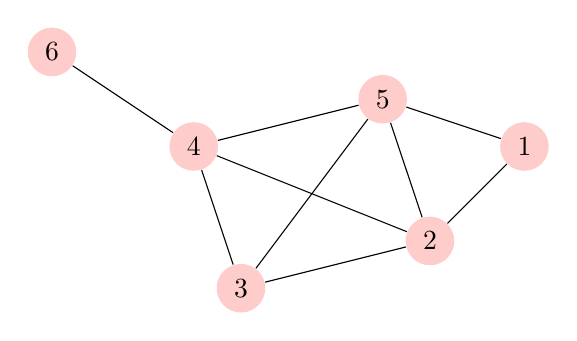
\begin{tikzpicture}
  [scale=.6,auto=left,every node/.style={circle,fill=red!20}]
  \node (n6) at (1,10) {6};
  \node (n4) at (4,8)  {4};
  \node (n5) at (8,9)  {5};
  \node (n1) at (11,8) {1};
  \node (n2) at (9,6)  {2};
  \node (n3) at (5,5)  {3};

  \foreach \from/\to in {n6/n4,n4/n5,n5/n1,n1/n2,n2/n5,n2/n3,n3/n4,n4/n2,n3/n5}
    \draw (\from) -- (\to);

\end{tikzpicture}
\caption{A graph with six vertices and nine edges for which we wish to identify the cliques, i.e.,~maximal complete subgraphs (there are three)}\label{13g1}
\end{center}
\end{figure}

Ajur was unsure of his answer, as he was struggling with all of the definitions. He said, ``If I understand correctly, there are three cliques:
\begin{enumerate}
    \item The induced subgraph containing vertices~4 and~6.
    \item The induced subgraph containing vertices~2, 3, 4, and~5.
    \item The induced subgraph containing vertices~1, 2, and~5.
\end{enumerate} 

Rishnak smiled. He was happy that Ajur understood. He said, ``Good, now how about for this graph?'' He waved his hands and four edges were added to the original graph to form a new graph [Figure~\ref{13g21}].

\begin{figure}
\begin{center}
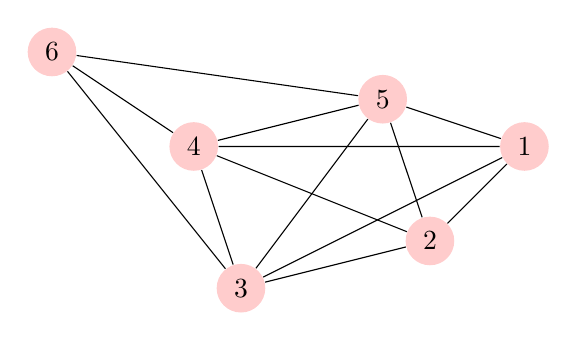
\begin{tikzpicture}
  [scale=.6,auto=left,every node/.style={circle,fill=red!20}]
  \node (n6) at (1,10) {6};
  \node (n4) at (4,8)  {4};
  \node (n5) at (8,9)  {5};
  \node (n1) at (11,8) {1};
  \node (n2) at (9,6)  {2};
  \node (n3) at (5,5)  {3};

  \foreach \from/\to in {n6/n4,n4/n5,n5/n1,n1/n2,n2/n5,n2/n3,n3/n4,n4/n2,n3/n5,n1/n4,n1/n3,n3/n6,n5/n6}
    \draw (\from) -- (\to);

\end{tikzpicture}
\caption{The graph shown in Figure~\ref{13g1} with four additional edges for which we again wish to identify the cliques (there are two)}\label{13g21}
\end{center}
\end{figure}

Ajur studied the graph for a few seconds, then answered, ``I think there are two cliques:
\begin{enumerate}
    \item The induced subgraph containing vertices~3, 4, 5, and~6.
    \item The induced subgraph containing vertices~1, 2, 3, 4, and~5.''
\end{enumerate}

Rishnak said, ``Exactly. Graphs are usually used as models for physical or social processes. For example, when we consider cliques in a school, we can model students as vertices and two students belong to the same group as an edge between the associated vertices, which also note forms a binary relation. Imagine a graph of everyone in your school, with a vertex for each student and an edge for each friendship.  Finding cliques or, as in the field of data science, finding clusters is an important task.''

Ajur thought about this for a few moments, trying to imagine a graph that would include all of his classmates at school.

Rishnak said, ``Let us move on to another related topic. An \textit{independent set} in a graph is a set of vertices that are mutually nonadjacent, which means that we have a subset of vertices that does not include any adjacent vertices. Can you see how an independent set is related to a clique?''

Ajur frowned, frustrated with the lesson so far. At length, Ajur said, ``No, I don't understand.''

Rishnak also frowned, thinking, ``Oh no, if Ajur does not understand and then does not answer my question, I will remain trapped as a ghost forever.''

Rishnak said, ``Let me give you a hint. A \textit{complement} of a graph~$G=(V,E)$ is another graph~$H=(V,E_1)$. Both have the same vertex set, but if two vertices are adjacent in~$G$, they are not adjacent in~$H$---and if two vertices are not adjacent in~$G$, then they are adjacent in~$H$. Can you draw the complement of the original graph''---he waved his hands and the four added edges disappeared to form the original graph [Figure~\ref{13g1}]---``in front of you?''

Ajur looked at the graph. He grabbed a stick and, after scratching his head a few times, drew a new graph in the dirt [Figure~\ref{13g2}]. He said, ``Here is the complement of your graph.''

Rishnak said, ``Yes, and how many edges will be in edge set~$E_1$ if the original graph has~$n$ vertices and~$e$ edges?''

Ajur said, ``The maximum number of edges a graph with~$n$ vertices can have is~$\frac{1}{2}n(n-1)$, so then the number of edges in the complement of the graph is simply~$\frac{1}{2}n(n-1)-e$.''

\begin{figure}
\begin{center}
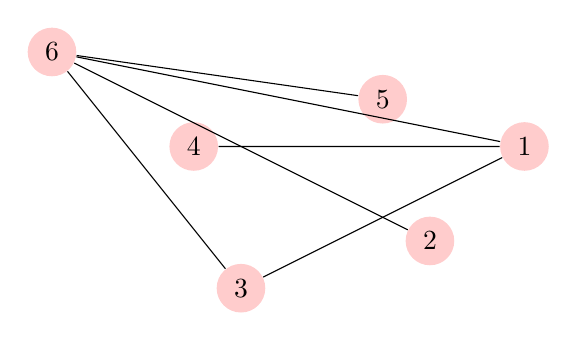
\begin{tikzpicture}
  [scale=.6,auto=left,every node/.style={circle,fill=red!20}]
  \node (n6) at (1,10) {6};
  \node (n4) at (4,8)  {4};
  \node (n5) at (8,9)  {5};
  \node (n1) at (11,8) {1};
  \node (n2) at (9,6)  {2};
  \node (n3) at (5,5)  {3};

  \foreach \from/\to in {n6/n5,n6/n3,n6/n2,n6/n1, n1/n3,n1/n4}
    \draw (\from) -- (\to);

\end{tikzpicture}
\caption{The complement of the graph shown in Figure~\ref{13g1}}\label{13g2}
\end{center}
\end{figure}

Rishnak said, ``Go on.''

Ajur thought for a minute. What was he missing? How did all of these concepts relate to one another?

Rishnak said, ``Well, Ajur, do you see it?''

At last, Ajur said, ``I do, yes, I see! A clique in a graph~$G$ will be an independent set in the 
complement of~$G$. In your original graph''---he pointed to the graph in the air in front of him [Figure~\ref{13g1}]---``the maximal independent sets are vertex sets~$\{2,3,4,5\}$, $\{1,2,5\}$, and~$\{4,6\}$. These are also the cliques!''

Rishnak smiled. He flashed his hands and a new graph appeared in the air in front of Ajur [Figure~\ref{13g3}]. Rishnak said, ``Here is a bipartite graph, Ajur. Can you figure out what the maximal independent sets are in this graph?''

Ajur studied the graph, then said, ``The maximal independent sets are vertex sets~$\{1,2\}$, $\{3,4,5,6\}$''---he hesitated, trying to find if there were any others--``and~$\{2,6\}$. I think that's all.''

\begin{figure}
\begin{center}
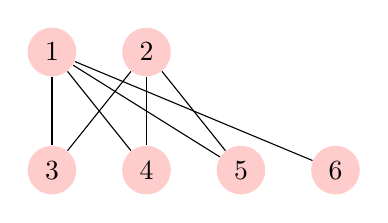
\begin{tikzpicture}
  [scale=.3,auto=left,every node/.style={circle,fill=red!20}]
  \node (n1) at (1,7) {1};
  \node (n2) at (5,7)  {2};
  \node (n3) at (1,2)  {3};
  \node (n4) at (5,2) {4};
  \node (n5) at (9,2)  {5};
   \node (n6) at (13,2) {6};
  
   \foreach \from/\to in {n1/n3,n1/n4,n1/n5,n2/n3,n2/n4,n2/n5,n1/n6}
    \draw (\from) -- (\to);
    \end{tikzpicture}
\caption{A bipartite graph with six vertices and seven edges for which we wish to find all of the maximal independent sets (there are three)}\label{13g3}
\end{center}
\end{figure}

Rishnak nodded. He said, ``Finding a maximal independent set is not that hard, but finding a \textit{maximum independent set} is very hard, similar to finding a maximum clique. And what I mean here is this. A maximum independent set refers to the maximal independent set with the largest size. For the graph you still see in front of you [Figure~\ref{13g3}], the maximum independent set is~$\{3,4,5,6\}$. And for this other graph''---Rishnak waved his hands and the previous graph appeared [Figure~\ref{13g2}]---''the maximum independent set is~$\{2,3,4,5\}$.''

Ajur said, ``Can we simplify the problem by just looking at a tree?''

Rishnak raised his eyebrows, pleased with Ajur's question.  He said, ``Yes, it is much easier to find the maximum independent set in a tree.  Can you come up with a procedure to do this?''

Ajur jumped up and thought for a few moments. Before long, he had a solution in mind. He said, ``First, the input is rooted tree~$T$ and the output is maximum independent set~$X$. The algorithm is:
\begin{enumerate}
    \item Let~$X=\emptyset$.\footnote{Here,~$\emptyset$ is the symbol for an empty set, also written as~$\{\}$.}
    \item Add all leaf vertices of~$T$ to set~$X$.
    \item Delete all leaf vertices from~$T$, meaning we also delete all edges incident to each of these leaf vertices.
    \item Next, delete all of the newly created leaf vertices, if any.
    \item If tree~$T$ is not empty, go back to Step~2.
    \item $X$ is the maximum independent set of tree~$T$.''
\end{enumerate}

Before Rishnak could say a word, Ajur excitedly drew a tree in the dirt [Figure~\ref{13g4}] and said, ``In this tree, the maximum independent set is vertex set~$\{4,5,6,7,1\}$.''

\begin{figure}
\begin{center}

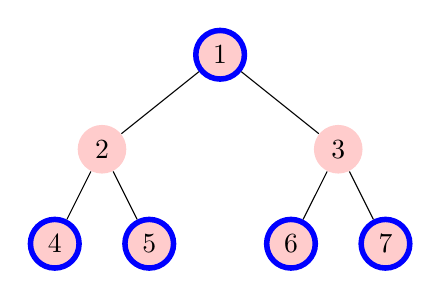
\begin{tikzpicture}
  [scale=.6,auto=left,every node/.style={circle,fill=red!20}]
  \tikzstyle{indset} = [draw=blue,line width=2pt]
  \node[indset] (n1) at (5.5,7) {1};
  \node (n2) at (3,5)  {2};
  \node (n3) at (8,5)  {3};
  \node[indset] (n4) at (2,3) {4};
  \node[indset] (n5) at (4,3)  {5};
  \node[indset] (n6) at (7,3)  {6};
  \node[indset] (n7) at (9,3)  {7};

  \foreach \from/\to in {n1/n2,n1/n3,n2/n4,n2/n5,n3/n6,n3/n7}
    \draw (\from) -- (\to);

\end{tikzpicture}
\caption{A tree for which the maximum independent set is vertex set~$\{4,5,6,7,1\}$, shown as circled vertices}\label{13g4}
\end{center}
\end{figure}

Rishnak said, ``A problem that is closely related to finding an independent set is finding what is called a \textit{vertex cover}. A vertex cover of a graph is a minimal subset of vertices that are incident to (or cover) all edges of the graph. In other words, if you delete all incident edges in a vertex cover, the remaining graph is always an empty graph, meaning a graph with no edges whatsoever.''

Ajur nodded and said, ``How is that useful?''

Rishnak said, ``Intuitively, if we place police officers at all vertices of the vertex cover, then they will be able to watch all of the edges, which may represent roadways in a city or corridors in a building. And since we want to employ as few police officers as possible, we want a minimal vertex cover, which here means that no subset of it is also a vertex cover.''

\begin{figure}
\begin{center}

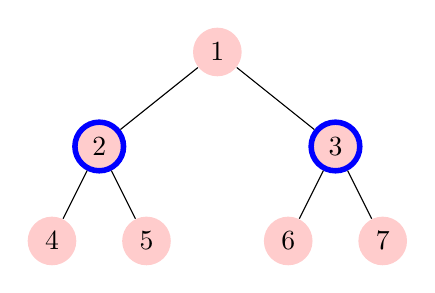
\begin{tikzpicture}
  [scale=.6,auto=left,every node/.style={circle,fill=red!20}]
  \tikzstyle{indset} = [draw=blue,line width=2pt]
  \node (n1) at (5.5,7) {1};
  \node[indset] (n2) at (3,5)  {2};
  \node[indset] (n3) at (8,5)  {3};
  \node (n4) at (2,3) {4};
  \node (n5) at (4,3)  {5};
  \node (n6) at (7,3)  {6};
  \node (n7) at (9,3)  {7};

  \foreach \from/\to in {n1/n2,n1/n3,n2/n4,n2/n5,n3/n6,n3/n7}
    \draw (\from) -- (\to);

\end{tikzpicture}
\caption{The tree from Figure~\ref{13g4} for which the minimal vertex cover is vertex set~$\{2,3\}$ (shown as circled vertices), as all edges are incident on either vertex~2 or vertex~3}\label{13g5}
\end{center}
\end{figure}

Ajur said, ``Vertex cover and independent set seem to be related. Are they?''

Rishnak smiled and replied, ``If~$X$ is a maximal independent set in a graph with~$V$ as its vertex set, then~$V-X$ is a minimal vertex cover. Similarly, if~$Y$ is a maximum independent set, then~$V-Y$ is a minimum vertex cover.''

Ajur smiled, seeing the elegance and simplicity. He also was impressed at how all of these seemingly unrelated sets were actually related. Ajur was lost in thought for awhile, then said, ``Maximal independent set~$X$ contains no edges, as per its definition. And this implies that vertex set~$V-X$ covers all edges of the graph and that every edge is incident in some vertex of~$V-X$.''

Rishnak said, ``In days long ago, parks were constructed at the junctions of roads in a village. Here is an old road map of Royt.'' Rishnak flashed his hands and a new graph appeared [Figure~\ref{13g6}]. He continued, ``What is the smallest number of parks that would need to be constructed in Royt such that there is at least a park at either end of each roadway or edge?''

\begin{figure}
\begin{center}

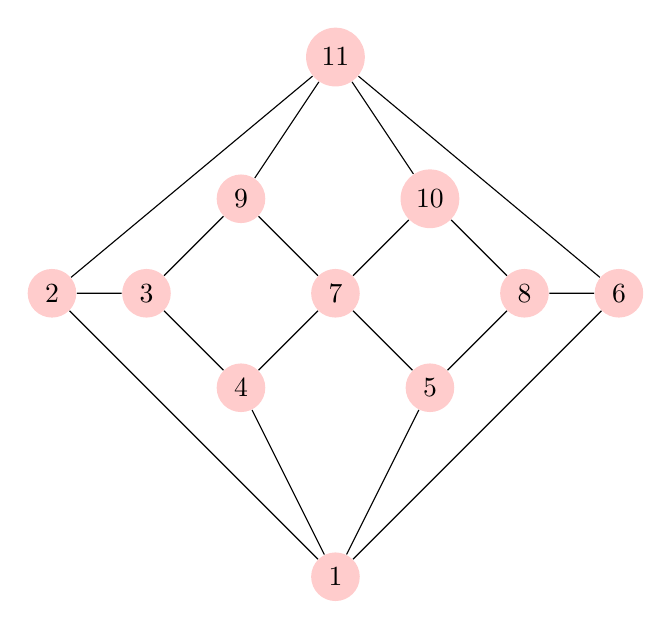
\begin{tikzpicture}
  [scale=.6,auto=left,every node/.style={circle,fill=red!20}]
  \node (n1) at (6,-3) {1};
  \node (n2) at (0,3)  {2};
  \node (n3) at (2,3)  {3};
  \node (n4) at (4,1) {4};
  \node (n5) at (8,1)  {5};
  \node (n6) at (12,3)  {6};
  \node (n7) at (6,3)  {7};
 \node (n8) at (10,3) {8};
  \node (n9) at (4,5)  {9};
  \node (n10) at (8,5)  {10};
  \node (n11) at (6,8)  {11}; 

  \foreach \from/\to in {n1/n2,n1/n4,n1/n5,n1/n6,n2/n3,n2/n11,n3/n4,n3/n9,n4/n7,n5/n7,n5/n8,n6/n8,n6/n11,n7/n9,n7/n10,n8/n10,n9/n11,n10/n11}
    \draw (\from) -- (\to);

\end{tikzpicture}
\caption{An old village road map of Royt}\label{13g6}
\end{center}
\end{figure}

Ajur was mesmerized by the almost ornate layout and symmetry of Royt. He studied the graph and said, ``I would construct five parks at vertices~1, 3, 7, 8, and~11.''

Rishnak raised his eyebrows and said, ``How did you come to that answer so quickly?''

Ajur said simply that he tried to find a minimum vertex cover to solve the problem.

\subsection*{Question for the eleventh day}
Rishnak smiled. He said, ``You are ready for the question for the eleventh day, Ajur. Here it is. What is the size of the maximum independent set in a complete binary tree of height~5?''

\textit{Before you turn the page, try to come up with answers of your own!}

\newpage
\subsection*{Answer for the eleventh day}
Ajur thought about the question, repeating it in his head. He said, ``Okay, a complete binary tree of height~5 will have 32~leaf vertices. From those leaf vertices, we go up the tree level by level, only counting vertices at alternating levels. So, the size of the maximum independent set will be~$32+8+2=42$.''

Rishnak was impressed, but before he could say good night, Ajur said, ``And the minimum vertex cover size is~$1+4+16=21$.''

Rishnak laughed.

It was getting dark and both of them called it a night.
